\documentclass[10pt,aspectratio=169]{beamer}
\usetheme{Madrid}
\usecolortheme{default}
\setbeamertemplate{navigation symbols}{}
\setbeamertemplate{footline}[frame number]

\usepackage[utf8]{inputenc}
\usepackage[T1]{fontenc}
\usepackage{amsmath,amssymb,amsthm}
\usepackage{tikz}
\usepackage{booktabs}
\usepackage{graphicx}
\usepackage{colortbl}
\usetikzlibrary{arrows.meta,positioning,fit,backgrounds}

\newcommand{\Inc}{\ensuremath{\mathrm{Inc}}}
\newcommand{\Exc}{\ensuremath{\mathrm{Exc}}}
\newcommand{\vbar}{\bar{v}}

\title{Une règle locale à quatre cas pour les machines de Tsetlin}
\subtitle{Analyse de convergence exacte et classifieur conditionné/boosté}
\author{Anaïs Hidouche}
\date{Réunion d'avancement}

\begin{document}

\begin{frame}
\titlepage
\end{frame}

\begin{frame}{Plan}
\tableofcontents
\end{frame}

% =====================================================================
\section{Analyse théorique}
% =====================================================================

\begin{frame}{La règle à quatre cas}
$(X_t,Y_t)_{t\ge1}\overset{\mathrm{iid}}{\sim}P$, $P(X,Y)$ arbitraire.

\begin{center}
\begin{tabular}{cccc}
\toprule
$x_i$ & $y$ & Action sur $v_i$ & Action sur $\vbar_i$ \\
\midrule
0 & 0 & vers $\Inc$ (proba $S$) & vers $\Exc$ (proba $S$) \\
0 & 1 & vers $\Exc$ (proba $a$) & -- \\
1 & 0 & vers $\Exc$ (proba $S$) & vers $\Inc$ (proba $S$) \\
1 & 1 & -- & vers $\Exc$ (proba $a$) \\
\bottomrule
\end{tabular}
\end{center}
\vspace{4mm}
\begin{itemize}
  \item $y=0$ : on cherche un littéral \emph{violé} par l'exemple négatif ($S$).
  \item $y=1$ : on exclut les littéraux \emph{incompatibles} avec l'exemple positif ($a$).
  \item \alert{Ne dépend que de $(x_i,y)$} -- pas de $C(x)$, pas du vote global.
\end{itemize}
\end{frame}

\begin{frame}{La chaîne d'un automate}
\begin{center}
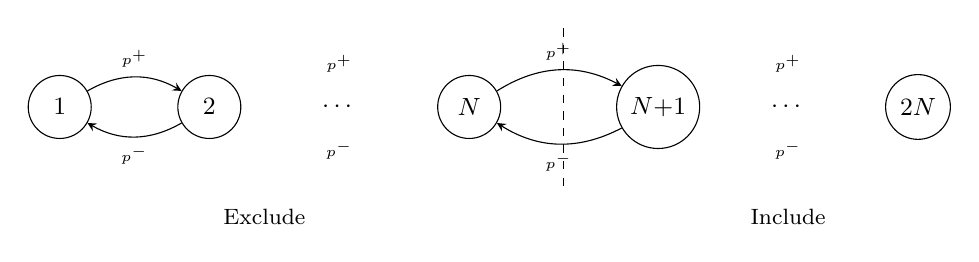
\begin{tikzpicture}[>=stealth, every node/.style={font=\small}, scale=1.0]
  \node[draw, circle, minimum size=8mm] (s1)  at (0,0)   {$1$};
  \node[draw, circle, minimum size=8mm] (s2)  at (1.9,0) {$2$};
  \node[draw, circle, minimum size=8mm] (sN)  at (5.2,0) {$N$};
  \node[draw, circle, minimum size=8mm] (sN1) at (7.6,0) {$N{+}1$};
  \node[draw, circle, minimum size=8mm] (s2N) at (10.9,0) {$2N$};
  \node at (3.55,0) {$\cdots$};
  \node at (9.25,0) {$\cdots$};
  % paire 1 <-> 2
  \draw[->] (s1) to[bend left=30] node[above,font=\tiny]{$p^+$} (s2);
  \draw[->] (s2) to[bend left=30] node[below,font=\tiny]{$p^-$} (s1);
  \node[font=\tiny] at (3.55,0.55) {$p^+$};
  \node[font=\tiny] at (3.55,-0.55) {$p^-$};
  % paire N <-> N+1 (frontiere)
  \draw[->] (sN) to[bend left=30] node[above,font=\tiny]{$p^+$} (sN1);
  \draw[->] (sN1) to[bend left=30] node[below,font=\tiny]{$p^-$} (sN);
  \node[font=\tiny] at (9.25,0.55) {$p^+$};
  \node[font=\tiny] at (9.25,-0.55) {$p^-$};
  \draw[dashed] (6.4,1.0) -- (6.4,-1.0);
  \node at (2.6,-1.4) {\footnotesize Exclude};
  \node at (9.25,-1.4) {\footnotesize Include};
\end{tikzpicture}
\end{center}
\vspace{2mm}
\begin{itemize}
  \item Chaîne de naissance--mort \textbf{homogène} : à chaque état intérieur,
  $p^+$ pousse vers Include, $p^-$ pousse vers Exclude ($p^+,p^->0$).
  \item Automate $v$ (littéral $x_i$) : $p^+=S\,P(0,0)$, $\
  p^-=S\,P(1,0)+a\,P(0,1)$, $\ \rho=p^+/p^-$.
  \item Automate $\bar v$ (littéral $\neg x_i$), \textbf{même chaîne},
  paramètres symétriques : $\bar p^+=S\,P(1,0)$, $\
  \bar p^-=S\,P(0,0)+a\,P(1,1)$, $\ \bar\rho=\bar p^+/\bar p^-$.
\end{itemize}
\end{frame}

\begin{frame}{Théorème 1 -- Loi stationnaire exacte}
\begin{block}{Théorème 1}
\footnotesize
Soit $p^+,p^->0$ et $\rho=p^+/p^-$. La chaîne $(v_t)$ est irréductible et
apériodique sur $\{1,\ldots,2N\}$, donc converge en loi vers l'unique loi
stationnaire
\[
  \pi(k) = \frac{(1-\rho)\rho^{k-1}}{1-\rho^{2N}}\ (\rho\ne1), \qquad
  \pi(\Inc) = \frac{\rho^N}{1+\rho^N}.
\]
\end{block}
\footnotesize
\textbf{Preuve.}
\begin{enumerate}
  \item \textbf{Irréductible} : transitions intérieures $p^+,p^->0$ dans les
  deux sens $\Rightarrow$ tout état atteint tout autre.
  \item \textbf{Apériodique} : l'état $1$ a une auto-boucle
  ($P(1,1)=1-p^+>0$) $\Rightarrow$ période $1$, donc toute la chaîne
  (irréductible) est apériodique.
  \item \textbf{Bilan détaillé} : $\pi(k)p^+=\pi(k{+}1)p^-\Rightarrow
  \pi(k{+}1)/\pi(k)=\rho$ constant, donc $\pi(k)=\pi(1)\rho^{k-1}$ ;
  normalisation $\sum_k\pi(k)=1$ (série géométrique) donne
  $\pi(1)=(1-\rho)/(1-\rho^{2N})$, d'où $\pi(k)$ ; puis
  $\pi(\Inc)=\sum_{k=N+1}^{2N}\pi(k)=\rho^N/(1+\rho^N)$. $\blacksquare$
\end{enumerate}
\alert{Convergence en loi}, pas stabilisation p.s. (sauf cas absorbant :
$p^+=0$ ou $p^-=0$). Si $\rho>1$ : $1-\pi(\Inc)\le\rho^{-N}$.
\end{frame}

\begin{frame}{Lemme de non-contradiction}
\textbf{Définitions} (dérives des automates $v$ et $\bar v$) :
\[
  \Delta := p^+-p^- = S\,P(0,0)-S\,P(1,0)-a\,P(0,1), \qquad
  \bar\Delta := \bar p^+-\bar p^- = S\,P(1,0)-S\,P(0,0)-a\,P(1,1).
\]
$\Delta>0$ signifie « $v$ est stationnairement poussé vers Include » (et
symétriquement pour $\bar\Delta,\bar v$).

\begin{block}{Lemme}
Pour toute loi $P(X,Y)$ : $\ \Delta+\bar\Delta=-a\,P(Y{=}1)\le0$.
$\Rightarrow$ jamais $\Delta>0$ et $\bar\Delta>0$ simultanément : la règle
ne peut pas favoriser stationnairement l'inclusion des deux littéraux
opposés ($x_i$ et $\neg x_i$) en même temps.
\end{block}

\textbf{Preuve.} La somme élimine les termes en $S$ :
$\Delta+\bar\Delta = -a\bigl[P(0,1)+P(1,1)\bigr] = -a\,P(Y{=}1) \le 0$,
avec égalité ssi $P(Y{=}1)=0$. $\blacksquare$

\vspace{1mm}
\textbf{Corollaire} : $\Delta>0 \Rightarrow \bar\Delta=-a\,P(Y{=}1)-\Delta<0$ strictement.
\end{frame}

\begin{frame}{Théorème des 3 régimes de sélection}
\footnotesize
\textbf{Sens des 3 régimes} ($\gamma=\max(\rho,1/\rho)>1$, $\bar\gamma$ idem pour $\bar v$) :
\begin{itemize}
  \item $\Delta>0$ (donc $\bar\Delta<0$, Lemme précédent) : à terme $v\to\Inc$, $\bar v\to\Exc$.
  \item $\bar\Delta>0$ (donc $\Delta<0$) : à terme $\bar v\to\Inc$, $v\to\Exc$.
  \item $\Delta<0$ et $\bar\Delta<0$ : à terme $v,\bar v\to\Exc$ (littéral neutre).
\end{itemize}

\begin{block}{Théorème}
\scriptsize
Exactement un des trois régimes a lieu :
\[
  \Delta>0 : \lim_N\limsup_t \mathbb P\bigl((v_t,\bar v_t)\ne(\Inc,\Exc)\bigr)=0 \quad\ \
  \bar\Delta>0 : \lim_N\limsup_t \mathbb P\bigl((v_t,\bar v_t)\ne(\Exc,\Inc)\bigr)=0
\]
\[
  \Delta<0 \text{ et } \bar\Delta<0 : \lim_N\limsup_t \mathbb P\bigl((v_t,\bar v_t)\ne(\Exc,\Exc)\bigr)=0
\]
\end{block}

\textbf{Preuve.}
\begin{enumerate}
  \item Chaque automate \emph{séparément} (Théorème 1) :
  $\limsup_t\mathbb P(v_t\ne\text{bon côté})\le\gamma^{-N}$ et
  $\limsup_t\mathbb P(\bar v_t\ne\text{bon côté})\le\bar\gamma^{-N}$.
  \item En sommant :
  \[
    \limsup_t \mathbb P\bigl((v_t,\bar v_t)\ne\text{bon régime}\bigr)
    \le \gamma^{-N}+\bar\gamma^{-N} \xrightarrow[N\to\infty]{} 0. \quad\blacksquare
  \]
\end{enumerate}
\end{frame}

\begin{frame}{Théorème -- Concentration structurelle multi-features}
\footnotesize
\textbf{Sens} : le Théorème des 3 régimes portait sur \emph{une} paire
$(v,\bar v)$. Ici on étend à toute une clause : $n$ features, $K$ fixées
par une condition, $d=n-K$ libres $\Rightarrow$ $2d$ automates à surveiller
\emph{en même temps}.

\begin{block}{Théorème}
\footnotesize
\[
  \limsup_{t\to\infty}\mathbb P(C_t\ne C^\star) \le \sum_{j=1}^{2d}\frac1{1+\gamma_j^N}
  \le 2(n-K)\,\gamma_{\min}^{-N}.
\]
\end{block}

\textbf{Preuve, en 3 points.}
\begin{enumerate}
  \item Soit $A_j$ : « l'automate $j$ est du mauvais côté ». Si tous les
  $A_j$ sont faux, alors $C_t=C^\star$ ; par contraposée,
  $\{C_t\ne C^\star\}\subseteq A_1\cup\cdots\cup A_{2d}$.
  \item $\mathbb P(C_t\ne C^\star)\le\sum_j\mathbb P(A_j)$, et
  chaque $\mathbb P(A_j)=1/(1+\gamma_j^N)$ exactement (Théorème 1).
  \item On majore chaque terme par le \textbf{maillon faible}
  $\gamma_{\min}=\min_j\gamma_j$ (l'automate le plus lent) : la somme des
  $2d$ termes donne $2(n-K)\,\gamma_{\min}^{-N}$. $\blacksquare$
\end{enumerate}
\end{frame}

\begin{frame}{Identification sous dépendance arbitraire}
\footnotesize
\textbf{Ce qu'on essaie de démontrer} : le Théorème des 3 régimes dit vers
quelle structure $C^\star$ la règle converge, mais pas si $C^\star$
correspond à la \emph{vraie} cible. Ici, on le montre -- sous des
conditions vérifiables, même si les features sont corrélées et
déséquilibrées.

\vspace{1mm}
\textbf{Cadre} : $C_{\mathrm{true}}(x)=\bigwedge_{J_+}x_j\wedge\bigwedge_{J_-}(1{-}x_j)$
(la vraie conjonction), $Y=C_{\mathrm{true}}(X)$, loi jointe
\textbf{quelconque} (corrélée, déséquilibrée). Pour chaque variable $j$ :
\[
  A_j{=}P(X_j{=}0,Y{=}0),\ B_j{=}P(X_j{=}1,Y{=}0),\ C_j{=}P(X_j{=}0,Y{=}1),\ D_j{=}P(X_j{=}1,Y{=}1).
\]

\begin{block}{Théorème 9}
\footnotesize
Si $A_j>B_j$ pour $j\in J_+$ (resp. $B_j>A_j$ pour $J_-$, encadrement pour
les non pertinents), alors $C^\star=C_{\mathrm{true}}$.
\end{block}

\textbf{Preuve (idée).} Pour $j\in J_+$ : $Y{=}1\Rightarrow X_j{=}1$, donc
$C_j=0$ et $\Delta_j$ se réduit à $S(A_j-B_j)$, positif ssi $A_j>B_j$. Le
Lemme de non-contradiction donne alors $\bar\Delta_j<0$
\emph{automatiquement} -- pas besoin de le vérifier séparément.
\end{frame}

% =====================================================================
\section{Classifieur complet}
% =====================================================================

\begin{frame}{Architecture du classifieur complet}
\begin{center}
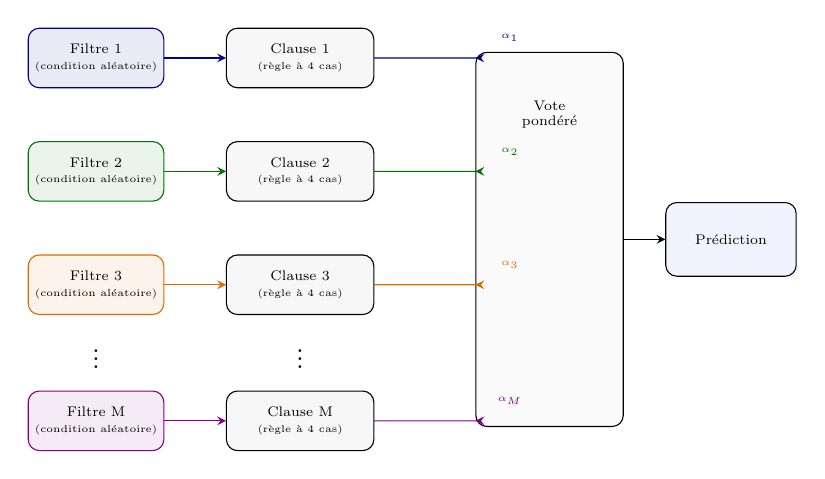
\begin{tikzpicture}[>=stealth, font=\scriptsize, scale=0.72, transform shape,
  every node/.style={font=\scriptsize}]
  \colorlet{c1}{blue!55!black}
  \colorlet{c2}{green!45!black}
  \colorlet{c3}{orange!85!black}
  \colorlet{c4}{violet}

  % Conditions column
  \foreach \i/\y/\col/\lbl in {1/4.2/c1/1, 2/2.2/c2/2, 3/0.2/c3/3, 4/-2.2/c4/M} {
    \node[draw, rounded corners, fill=\col!8, draw=\col, minimum width=2.1cm, minimum height=1.05cm, align=center]
      (cond\i) at (0,\y) {Filtre \lbl\\ \tiny (condition aléatoire)};
  }
  \node at (0,-1.0) {\Large $\vdots$};

  % Clause column
  \foreach \i/\y/\col/\lbl in {1/4.2/c1/1, 2/2.2/c2/2, 3/0.2/c3/3, 4/-2.2/c4/M} {
    \node[draw, rounded corners, fill=gray!6, minimum width=2.6cm, minimum height=1.05cm, align=center]
      (clause\i) at (3.6,\y) {Clause \lbl\\ \tiny (règle à 4 cas)};
    \draw[->, color=\col] (cond\i) -- (clause\i);
  }
  \node at (3.6,-1.0) {\Large $\vdots$};

  % Aggregation
  \node[draw, rounded corners, minimum width=2.6cm, minimum height=6.6cm, align=center, fill=gray!4]
    (agg) at (8.0,1.0) {};
  \node at (8.0,3.2) {\shortstack{Vote\\pondéré}};
  \foreach \i/\y/\col/\lbl in {1/4.2/c1/1, 2/2.2/c2/2, 3/0.2/c3/3, 4/-2.2/c4/M} {
    \draw[->, color=\col] (clause\i) -- (6.7,\y) -- (agg.west |- 6.7,\y);
    \node[color=\col] at (7.3,\y+0.35) {\tiny $\alpha_\lbl$};
  }

  \node[draw, rounded corners, minimum width=2.3cm, minimum height=1.3cm, align=center, fill=blue!5]
    (pred) at (11.2,1.0) {Prédiction};
  \draw[->] (agg) -- (pred);
\end{tikzpicture}
\end{center}
\footnotesize
\begin{itemize}
  \item Chaque clause n'est active que si $x$ satisfait son filtre (condition
  aléatoire) -- sinon elle s'abstient.
  \item Chaque clause active vote « oui »/« non », pondéré par sa fiabilité $\alpha_m$.
  \item On additionne tous les votes actifs ; le signe du total donne la
  prédiction.
\end{itemize}
\end{frame}

\begin{frame}[fragile]{Algorithme (une classe, one-vs-rest)}
\footnotesize
\begin{verbatim}
w_i <- 1/|train|
pour m = 1 a M :
    tirer F_m (K features), z_m (config binaire)
    geler les automates de F_m (Exclude, non entraines)
    S_m <- {i : x_i[F_m] = z_m}
    si S_m vide : alpha_m <- 0 ; continuer
    pour t = 1 a total :
        tirer i in S_m selon Q_m (50/50 classe, ~ w_i)
        mettre a jour C_m avec (x_i, 1[y_i=c])  (regle 4 cas)
    si C_m vide : alpha_m <- 0 ; continuer
    err_m <- erreur ponderee de C_m sur S_m (sous D_m)
    alpha_m <- 1/2 ln((1-err_m)/err_m)
    mettre a jour w (exp(+-alpha_m)) ; renormaliser
\end{verbatim}
\end{frame}

% =====================================================================
\section{Résultats empiriques}
% =====================================================================

\begin{frame}{Résultats principaux}
\begin{center}
\small
\begin{tabular}{lccc}
\toprule
Dataset & Notre modèle & TM officielle & Meilleure baseline \\
\midrule
XOR    & $\mathbf{100\%\pm0\%}$ & $97.40\%\pm2.23\%$ & SVM $98.12\%$ \\
Iris   & $95.5\%$ & $93.50\%$ & RF $95.33\%$ \\
Digits & $97.19\%$ & $93.69\%$ & SVM $97.50\%$ \\
MNIST  & $95.85\%$ (1 run) & $96.62\%$ & SVM $97.71\%$ \\
\bottomrule
\end{tabular}
\end{center}
\vspace{3mm}
\begin{itemize}
  \item XOR : net, mais budgets non égalisés (clauses différentes).
  \item MNIST : en dessous de la TM et des baselines classiques -- honnête,
  un seul run à $M{=}16000$ (limite reconnue).
\end{itemize}
\end{frame}

\begin{frame}{Balayage $S,\alpha$ -- XOR}
\begin{center}
\renewcommand{\arraystretch}{1.15}
\begin{tabular}{cccccccc}
\toprule
$S \backslash \alpha$ & 0,1 & 0,3 & 0,35 & 0,5 & 0,7 & 0,9 & 1,0 \\
\midrule
0,1 & 78,1 & \cellcolor{red!15}48,9 & \cellcolor{red!15}48,9 & \cellcolor{red!15}48,9 & \cellcolor{red!15}48,9 & \cellcolor{red!15}48,9 & \cellcolor{red!15}48,9 \\
0,3 & 86,1 & 74,2 & 64,3 & \cellcolor{red!15}48,9 & \cellcolor{red!15}48,9 & \cellcolor{red!15}48,9 & \cellcolor{red!15}48,9 \\
0,5 & 85,4 & 91,5 & 82,7 & 61,6 & \cellcolor{red!15}48,9 & \cellcolor{red!15}48,9 & \cellcolor{red!15}48,9 \\
0,7 & 84,1 & 95,8 & 89,0 & 77,0 & 51,4 & \cellcolor{red!15}48,9 & \cellcolor{red!15}48,9 \\
0,9 & 81,9 & 97,5 & 95,8 & 80,1 & 69,4 & \cellcolor{red!15}48,9 & \cellcolor{red!15}48,9 \\
1,0 & 81,1 & 98,6 & \textbf{99,1} & 83,4 & 75,8 & 56,5 & \cellcolor{red!15}48,9 \\
\bottomrule
\end{tabular}
\end{center}
\end{frame}

\begin{frame}{Balayage $S,\alpha$ -- Iris}
\begin{center}
\renewcommand{\arraystretch}{1.15}
\begin{tabular}{ccccccc}
\toprule
$S \backslash \alpha$ & 0,05 & 0,1 & 0,3 & 0,5 & 0,7 & 1,0 \\
\midrule
0,05 & 95,5 & 92,0 & 89,8 & 88,0 & 88,0 & 88,2 \\
0,1  & 95,5 & 95,7 & 90,7 & 90,7 & 89,3 & 88,0 \\
0,3  & 95,5 & 95,5 & 95,3 & 90,8 & 92,0 & 91,8 \\
0,5  & 95,5 & 95,5 & 95,5 & 94,8 & 92,8 & 92,2 \\
0,7  & 95,5 & 95,5 & 95,5 & 95,5 & 95,2 & 92,8 \\
1,0  & 95,5 & 95,5 & 95,5 & 95,5 & 95,5 & \textbf{95,7} \\
\bottomrule
\end{tabular}
\end{center}
\end{frame}

\begin{frame}{Balayage $S,\alpha$ -- Digits}
\begin{center}
\renewcommand{\arraystretch}{1.15}
\begin{tabular}{ccccccc}
\toprule
$S \backslash \alpha$ & 0,05 & 0,1 & 0,3 & 0,5 & 0,7 & 1,0 \\
\midrule
0,05 & 95,6 & 95,8 & 96,5 & 96,4 & 96,4 & \textbf{97,1} \\
0,1  & 95,6 & 95,6 & 95,8 & 96,5 & 96,9 & 96,5 \\
0,3  & 95,6 & 95,6 & 95,4 & 96,0 & 96,0 & 96,8 \\
0,5  & 95,6 & 95,6 & 95,4 & 95,6 & 95,0 & 96,3 \\
0,7  & 95,6 & 95,6 & 95,4 & 95,6 & 95,3 & 95,0 \\
1,0  & 95,6 & 95,6 & 95,4 & 95,6 & 95,6 & 94,2 \\
\bottomrule
\end{tabular}
\end{center}
\end{frame}

\begin{frame}{Balayage $S,\alpha$ -- MNIST}
\begin{center}
\renewcommand{\arraystretch}{1.15}
\begin{tabular}{ccccccc}
\toprule
$S \backslash \alpha$ & 0,05 & 0,1 & 0,3 & 0,5 & 0,7 & 1,0 \\
\midrule
0,05 & 85,9 & 80,5 & 58,4 & 52,7 & 51,0 & 39,6 \\
0,1  & 85,9 & 85,9 & 71,5 & 58,1 & 51,7 & 48,8 \\
0,3  & 85,9 & 85,9 & 85,9 & 77,4 & 71,7 & 63,7 \\
0,5  & 85,9 & 85,9 & 85,9 & 85,9 & 79,7 & 74,2 \\
0,7  & 85,9 & 85,9 & 85,9 & 85,9 & 85,9 & 78,8 \\
1,0  & 85,9 & 85,9 & 85,9 & 85,9 & 85,9 & \textbf{85,5} \\
\bottomrule
\end{tabular}
\end{center}
\end{frame}

\end{document}
